\documentclass{article}

\usepackage{fullpage}
\usepackage{color}
\usepackage{amsmath}
\usepackage{url}
\usepackage{verbatim}
\usepackage{graphicx}
\usepackage{parskip}
\usepackage{amssymb}
\usepackage{nicefrac}
\usepackage{listings} % For displaying code
\usepackage{algorithm2e} % pseudo-code

\usepackage{subcaption}
\usepackage[usenames,dvipsnames]{xcolor}

\newcommand{\vect}[1]{\boldsymbol{#1}}
\newcommand\R{\mathbb R}
\newcommand\K{\vect{K}}

%%
%% Julia definition (c) 2014 Jubobs
%%
\lstdefinelanguage{Julia}%
{morekeywords={abstract,break,case,catch,const,continue,do,else,elseif,%
		end,export,false,for,function,immutable,import,importall,if,in,%
		macro,module,otherwise,quote,return,switch,true,try,type,typealias,%
		using,while,begin},%
	sensitive=true,%
	alsoother={\#},%
	morecomment=[l]\#,%
	morecomment=[n]{\#=}{=\#},%
	morestring=[s]{"}{"},%
	morestring=[m]{'}{'},%
}[keywords,comments,strings]%

\lstset{%
	language         = Julia,
	basicstyle       = \ttfamily,
	keywordstyle     = \color{blue},
	stringstyle      = \color{magenta},
	commentstyle     = \color{ForestGreen},
	showstringspaces = false,
}

% Answers
\def\ans#1{\par\gre{Answer: #1}}
%\def\ans#1{} % Comment this line to produce document with answers

% Colors
\definecolor{blu}{rgb}{0,0,1}
\def\blu#1{{\color{blu}#1}}
\definecolor{gre}{rgb}{0,.5,0}
\def\gre#1{{\color{gre}#1}}
\definecolor{red}{rgb}{1,0,0}
\def\red#1{{\color{red}#1}}
\def\norm#1{\|#1\|}

% Math
\def\R{\mathbb{R}}
\def\argmax{\mathop{\rm arg\,max}}
\def\argmin{\mathop{\rm arg\,min}}
\newcommand{\mat}[1]{\begin{bmatrix}#1\end{bmatrix}}
\newcommand{\alignStar}[1]{\begin{align*}#1\end{align*}}
\def\half{\frac 1 2}
\def\cond{\; | \;}

% LaTeX
\newcommand{\fig}[2]{\includegraphics[width=#1\textwidth]{a2f/#2}}
\newcommand{\centerfig}[2]{\begin{center}\includegraphics[width=#1\textwidth]{a2f/#2}\end{center}}
\def\items#1{\begin{itemize}#1\end{itemize}}
\def\enum#1{\begin{enumerate}#1\end{enumerate}}


\begin{document}
	\title{Visualization tools for understanding secondary structure effects on DNA reaction kinetics \vspace{-0.7em}}
	\author{Chenwei Zhang}
	\date{}
	\maketitle
	\vspace{-3em}



\section*{Introduction and related work}

Nucleic acids, namely deoxyribonucleic acid (DNA) and ribonucleic acid (RNA), play important roles in the continuity of life. DNA exists in almost every organism and carries genetic information and instructions on protein synthesis. RNA molecules involving three major types such as transfer RNA (tRNA), messenger RNA (mRNA), and ribosomal RNA (rRNA) are mainly functionalized to convert information stored in DNA into proteins. In the past few decades, DNA and RNA nanotechnologies have been developed that are capable of sensing and responding to changes in their environments, self-assembling into complex structures, and simulating computational models such as logic circuits or artificial neural networks. Thermodynamics of nucleic acids has been extensively studied, but the mechanisms that influence DNA reaction kinetics are less well understood. There are multiple simulation tools available for this purpose, including \textit{Multistrand} \cite{Schaeffer,multistrandpaper}, \textit{Kinfold} \cite{Kinfold}, \textit{Kfold} \cite{Kfold}, and \textit{oxDNA} \cite{oxDNA}. But there is also a need for better visualization techniques that can make the output of the simulation tools more comprehensible to domain experts. This project will focus on implementing powerful graphing tools to visualize nucleic acid reaction kinetics. 


\textit{Multistrand} \cite{Schaeffer,multistrandpaper}, \textit{Kinfold} \cite{Kinfold}, and \textit{Kfold} \cite{Kfold} use continuous-time Markov Chains (CTMCs) to model nucleic acid kinetics. A CTMC model of a reaction consists of a set of states corresponding to secondary structures, plus transitions, and transition rates between states. A secondary structure describes the set of base pairs formed via hydrogen bonding between Watson-Crick complementary bases, and each state has an associated free energy that is determined by latent thermodynamic parameters. Each elementary step corresponds to a single base pair forming or breaking, and the elementary step rates are determined by the state free energies as well as latent kinetic parameters. Roughly, transitions that lead to lower-energy states are more likely than those that increase the free energy. A CTMC with reasonable space size can offer direct computation of its dynamics with matrix equations. However, CTMCs that model typical DNA or RNA reactions of interest often have a prohibitively large state space size. Therefore, it is infeasible to enumerate all the states to compute measures over paths. As a result, appropriate sampling approaches, such as the Gillespie sampling algorithm \cite{Gillespie} have to be applied to simulate statistically correct trajectories, i.e., sequences of observed states (secondary structures) along with the time for each transition \cite{Schaeffer}.

One example of an important DNA reaction is toehold-mediated three-way strand displacement, see Figure \ref{fig:threeway}. An invader strand initially binds to unpaired bases of a substrate strand, and then, through a process called branch migration, forms more base pairs with the substrate, displacing the incumbent strand in the process. The rate of the process depends in part on whether the invader is a perfect Watson-Crick complement to the region of the substrate to which it binds, or whether there is a mismatched base, and furthermore on the position of such a mismatch \cite{MachinekThreeway}.

There are really two different challenges with respect to showcasing nucleic acid reactions based on their CTMCs or sampled trajectories. One is visualizing energy landscapes. The other is visualizing trajectories through those landscapes. One of the most basic visualizations just uses ``dot-parenthesis" notation to represent a secondary structure and a sequence of such strings to represent a trajectory. This method does not situate the trajectory in the overall energy landscape. Visualizations of energy landscapes use mappings of the high-dimensional state space to 2D or 3D. One example, for toehold-mediated three-way strand displacement, is shown in Figure \ref{fig:PElandscape}: the two dimensions show the number of base pairs between the substrate and incumbent, and the substrate and invader \cite{MachinekThreeway}. However, this visualization is very specific to the underlying reaction. Flamm et al. use barrier trees to visualize landscapes. This approach is distinctive but does not provide a way to visualize trajectories through such landscapes \cite{barriertrees,Badelt}. Castro et al. \cite{deepgraph} use deep graph embedding techniques to uncover the energy landscape of DNA secondary structure. However, this approach does not address how to visualize trajectories through those landscapes and the output of deep graph embedding approaches may not be at all intuitive to researchers in DNA nanotechnology. \textit{Kinefold} generates a movie showing reaction kinetics but is limited to displaying one trajectory, and does not show the overall energy landscape \cite{kinefold}. Accordingly, there is a need to have more visualization tools to visualize kinetic trajectories. Apart from sequence-level analysis, Berleant et al. \cite{domaincoarse} provide a domain-level based coarse-graining tool to display kinetic pathways, which is considered as an important reference for this project. The book \textit{Visualization Analysis and Design} \cite{tamara} related to the principles and implementations of visualization is also a good reference for this project and I will spend some time to get through it during the project.

%To analyze DNA kinetics, we are interested in studying its secondary structure which indicates the hydrogen bonding state of the bases within the strand (i.e. base pairing). Based on this, five common types of DNA reactions are covered in the design of biosensors and DNA programming as shown in Figure \ref{fig:reactiontype}. For example, hairpin reactions refer to a single strand hybridizes itself to form or break a hairpin loop; bubble closing, helix association and dissociation, toehold-mediated three-way strand displacement, and toehold-mediated four-way strand exchange. Bubble closing is the base of a bubble form a fully hybridized domain. Helix association and dissociation refer to a duplex forming and breaking with two separate strand. And toehold-mediated three- and four-way strand reactions involve more than three strands to hybridize with each other.

There are many other interesting types of DNA reactions, in addition to toehold-mediated strand displacement shown in Figure \ref{fig:threeway}. While my work will be guided by common examples, my goal is to develop visualization tools that will also work more generally, and will help domain experts appreciate the mechanisms behind reaction kinetics.

%Among these reactions, however, few work has been done to analyze the influence of hairpins formation on reaction rates and pathways in DNA hybridization. Although there is an existing work provides insights on a few examples by using \textit{oxDNA} which is a coarse-grained model simulating nucleic acid nanotechnology \cite{oxDNA} to simulate hairpin structures in the duplex formation and study their effects on forward and backward reaction rates \cite{schreck}, it is still not clear whether hairpins affect the rates of helix association and disassociation on other DNA strands in the same way. Here, I propose a more straightforward way to reveal this process by implementing visualization tools to help domain experts to appreciate mechanisms behind the kinetics and help them to design deliberate molecular structures upon DNA nanotechnology.

\begin{figure}[h]
	\centering
	\vspace*{0.3cm}
	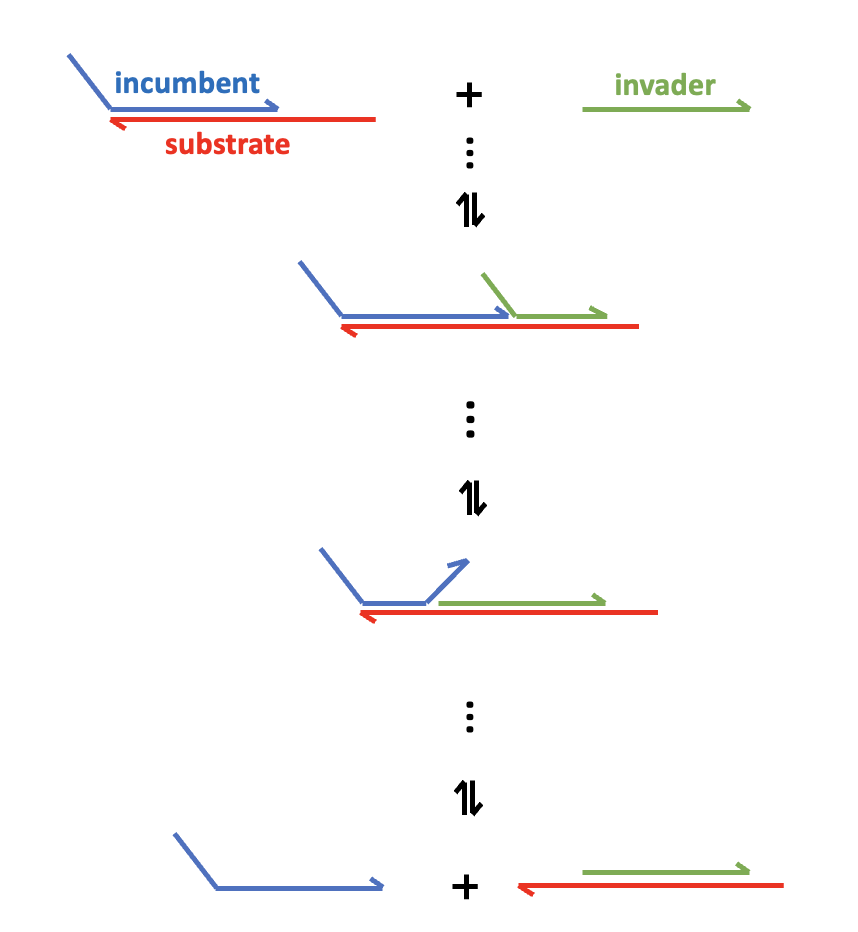
\includegraphics[scale=0.5]{latexplots/Threewayrxn.png}\hspace*{1cm}
	\caption{A toehold-mediated three-way strand displacement reaction and its mechanism. An invader strand (green line) replaces one of the strands in a duplex, i.e. incumbent strand (blue line), and forms a new double-helix strand with the substrate strand (red line). This figure shows a coarse-grained representation of the reaction, i.e. it groups many elementary steps into one coarse-grained step.}
	\vspace*{-.3cm}
	\label{fig:threeway}
\end{figure}


\begin{figure}[h]
	\centering
	\vspace*{0.3cm}
	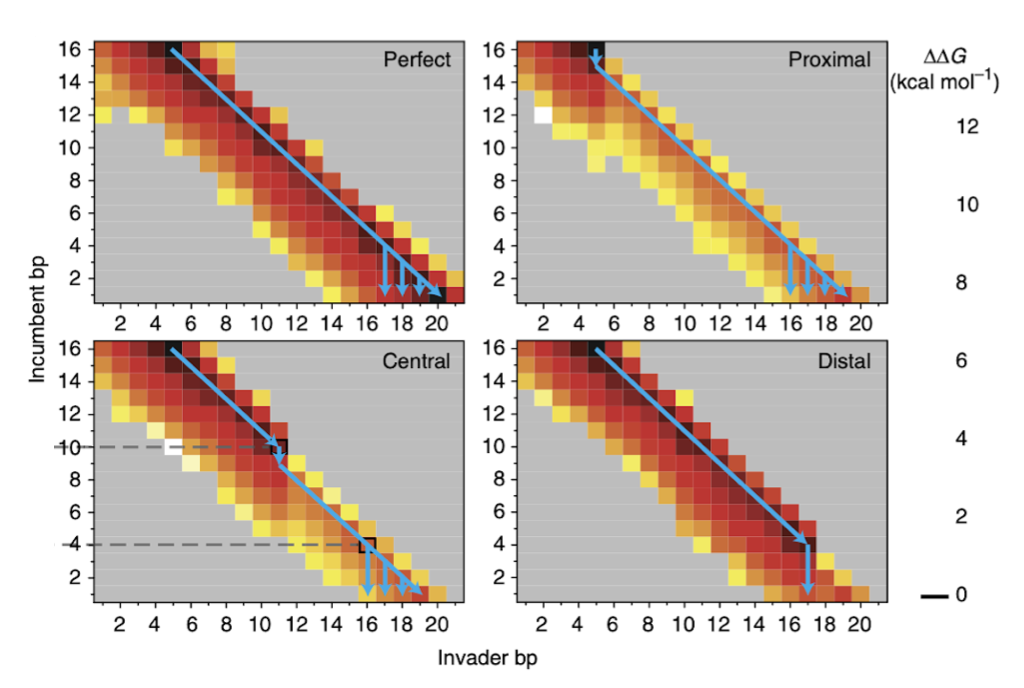
\includegraphics[scale=0.6]{latexplots/Machinek.png}\hspace*{1cm}
	\caption{Results of simulation of toehold-mediated three-way strand displacement without (top left panel) and with different kinds of mismatches (the rest of three panels). For these plots, coordinates represent the numbers of base pairs formed between the substrate and incumbent, and the substrate and invader. This figure is retrieved from \cite{MachinekThreeway}.}
	\vspace*{-.3cm}
	\label{fig:PElandscape}
\end{figure}


%
%\begin{figure}[h]
%	\centering
%	\vspace*{0.3cm}
%	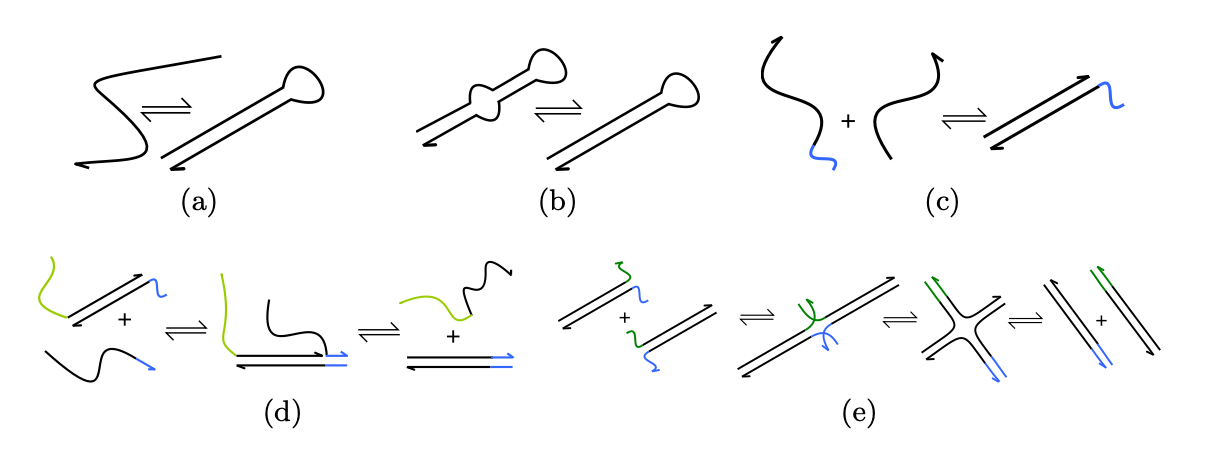
\includegraphics[height=3cm]{latexplots/dnareactiontypes.png}\hspace*{1cm}
%	\caption{Five common types of DNA reactions \cite{DNA23}.
%		\textbf{(a)} Hairpin closing and opening.
%        \textbf{(b)} Bubble closing.
%        \textbf{(c)} Helix association and dissociation.
%        \textbf{(d)} Toehold-mediated three-way strand displacement.
%        \textbf{(e)} Toehold-mediated four-way strand exchange.  }
%	\vspace*{-.3cm}
%	\label{fig:reactiontype}
%\end{figure}



%\section{Background on CTMCs}
%A CTMC is defined as a tuple $C = (S, \K, \pi_0, F)$, where $S$ refers to the set of states, $\K : S\times S \to \R_{\ge 0}$ refers to the rate matrix subject to $\K(s,s) = 0$ for any $s\in S$,  $\pi_0 : S\to [0,1]$ refers to the initial state distribution subject to $\sum_{s\in S} \pi_0(s) = 1$, and $F \subset S$ refers to the set of target (absorbing) states. We define $I \subset S$ as the set of initial states, that is $I = \{ s\in S \, | \, \pi_0(s) > 0\}$. A transition from states $s$ to $s'$ is possible only if $\K(s,s') > 0$. The exit rate matrix, $\vect{E} : S \times S \to \R_{\ge 0}$, is a diagonal matrix defined as $\vect{E} = \sum_{s'\in S} \K(s,s')$ in which each entry represents an exit rate. And the holding time of a state $s$ is exponentially distributed with respect to its corresponding exit rate $\vect{E}(s,s)$. We also define the generating matrix, $\vect{Q} : S\times S \to \R$, as $\vect{Q} = \K-\vect{E}$.

%A trajectory is denoted by $(s_0,t_0)$, $(s_1,t_1)$, ..., $(s_n,t_n)$ with n transitions over a CTMC model, where states $s_i$ and holding time $t_i$ subject to $\K(s_i,s_{i+1}) > 0$ and $t_i \in \R_{\geq 0}$ for $i \geq 0$. A path is defined as $s_0$, $s_1$, ..., $s_n$ with n transitions over a CTMC model, where states $s_i$ subject to $\K(s_i,s_{i+1}) > 0$. 

%\section*{Literature reviews}
%Here I list some related literatures that I will dig deeper into when start the project.
%\begin{enumerate}
%	\item Use kinefold
%	\item Use the barrier trees to visualize landscapes. This approach is distinctive but it does not graph trajectories \cite{barriertrees}.
%	\item Use graph embedding
%\end{enumerate}


\section*{Goals}
To summarize, in this project I am planning to :
\begin{enumerate}
	\item Review the literature. Here I list some related literature that I will dig deeper into when I start the project.
		\begin{enumerate}
			\item 2D or 3D embedding and projections papers \cite{deepgraph,PHATE,Manifold,projlandscape}.
			\item Case study papers \cite{domaincoarse,zhang2007,cotranscriptional,rnamovie,DSD}.
			\item Barrier trees papers \cite{barriertrees,Badelt}.
			\item The book \textit{Visualization Analysis and Design} \cite{tamara}.
		\end{enumerate}
	\item Develop visualization tools using Python and Julia. \\
	Here I list three possible options for designing visualization tools. Eventually I will choose one of the most interest to pursue further study.
		\begin{enumerate}
			\item 2D or 3D embeddings on a coarse-grained landscape. I am interested in generalizing this approach to other types of reaction including, but not limited to, those in \cite{DNA23}.
			\item Base pairing probabilities over time. 2D plots showing equilibrium base pairing probabilities are familiar to domain experts. The idea is to show these over time (add a slider).
			\item Possibly barrier trees. I may try to modify this visualization approach to show a pathway representation. 
		\end{enumerate}
	\item Evaluate the visualization tools using one or two case studies. 
	\begin{enumerate}
		\item Visualize kinetic pathways on two examples from the papers: Schreck et al. \cite{schreck} and Zhang et al. \cite{zhang2007}.
		\item Use \textit{Multistrand} to generate trajectories (or CTMCs, using pathway elaboration) if applicable, or augment the DNA23 collection of CTMCs to include helix association and dissociation with intermediate hairpin formation.
	\end{enumerate}
	
%	
%In this project, I aim to implement a meaningful graphing tool to visualize DNA hybridization kinetics, particularly helix association and dissociation processes and further to understand the effects on hairpins forming and breaking on the course of DNA double-helical strands hybridization and melting. To achieve this goal, I propose a 3D visualization tool with a time slider to display the secondary structure transformation between initial and final states, accompanying by hairpin structure forming and breaking. I am planning to implement Python and Julia to deal with datasets and make plots.
	
	
%		\item Implementation of different sampling methods, including Gillespie sampling, WES, FFS, and KPS to efficiently obtain statistically correct states and trajectories in large CTMCs.   
%	\item Find a meaningful way to index each state and design efficient visualization tools to understand the effect of hairpin structures on DNA hybridization.
%	\item If possible, get insights from Deep Graph Embeddings paper and then find common ground to combine my project with that approach \cite{deepgraph}.
%	\item If time permits, implement the pathway elaboration algorithm \cite{PE} and combine it with visualization tools to analyze the relationship between truncated states and hairpin secondary structures in helix association and dissociation.
\end{enumerate}


\section*{Challenges}
There are several challenges in this work.
\begin{enumerate}
	\item Find meaningful ways to index each state.
	\item How to show multiple trajectories through the landscapes.
	\item How to assess which visualization approach works better? One obvious way is domain experts' evaluation. Other assessing ways may resort to some insights from the visualization book \cite{tamara}.
\end{enumerate}


\section*{Timeline}
\begin{itemize}
	\item 1-Jun to 30-Jun: Review past works.
	\item 1-Jun to 15-Jul: Identify strengths and weaknesses of different possible visualization methods, and implement one of the more promising options.
	\item 16-Jul to 31-Aug: Evaluate the implemented tool(s) using case studies.
	\item 1-Sep to 30-Sep: Improve methods and write final report.
\end{itemize}


In conclusion, in this project I aim to design and implement general visualization tools for nucleic acid kinetics to help domain experts to make the output from the simulation approaches more comprehensible.


\clearpage
\bibliographystyle{unsrt}
{\bibliography{references.bib}}


\end{document}